% !TEX encoding = UTF-8 Unicode
\documentclass[aspectratio=1610,table,xcolor=dvipsnames]{beamer}


% Beamer Theme
\usetheme[]{mci} 


% Packages
\usepackage[utf8]{inputenc}
\usepackage{times}
\usepackage{multirow}
\usepackage{stmaryrd}
\usepackage{tikzsymbols}
\usepackage{subcaption}
%\usepackage{fontawesome}


\newenvironment<>{varblock}[2][.9\textwidth]{%
\setlength{\textwidth}{#1}
\begin{actionenv}#3%
	\setbeamerfont{varblock body}{size=\tiny}
    \def\insertblocktitle{#2}%
    \par%
    \usebeamertemplate{block begin}}
  {\par%
    \usebeamertemplate{block end}%
  \end{actionenv}}



%\overfullrule=5pt
\pgfplotsset{compat=1.15}

%%%%%%%%%%%%%%%%%%%%%%%%%%%%%%%%%%%%%%%%%%%%%%%%%%%%

% Titlepage Information
\title{Adversarial Examples Against a BERT ABSA Model}
\subtitle{Fooling Bert With L33T, Misspellign, and Punctuation,}

\author{N. Hofer, P. Schöttle, A. Rietzler, S. Stabinger} 
\date{August, 2021}
%\conference{16th International Conference on Availability, Reliability and Security (ARES 2021)}


%%%%%%%%%%%%%%%%%%%
%% Begin Document%%
%%%%%%%%%%%%%%%%%%%
\begin{document}
\setbeamertemplate{caption}{\raggedright\insertcaption\par}




% Titlepage
\begin{frame}
	\titlepage
\end{frame}



%BERT
\begin{frame}
	\frametitle{Motivation}
	\framesubtitle{Adversarial Examples Against a \textbf{BERT} ABSA Model}
	Bidirectional Encoder Representations from Transformers - BERT
	% \begin{figure}
	% 	\centering
	% 	\begin{subfigure}{.8\textwidth}
	% 		\centering
	% 		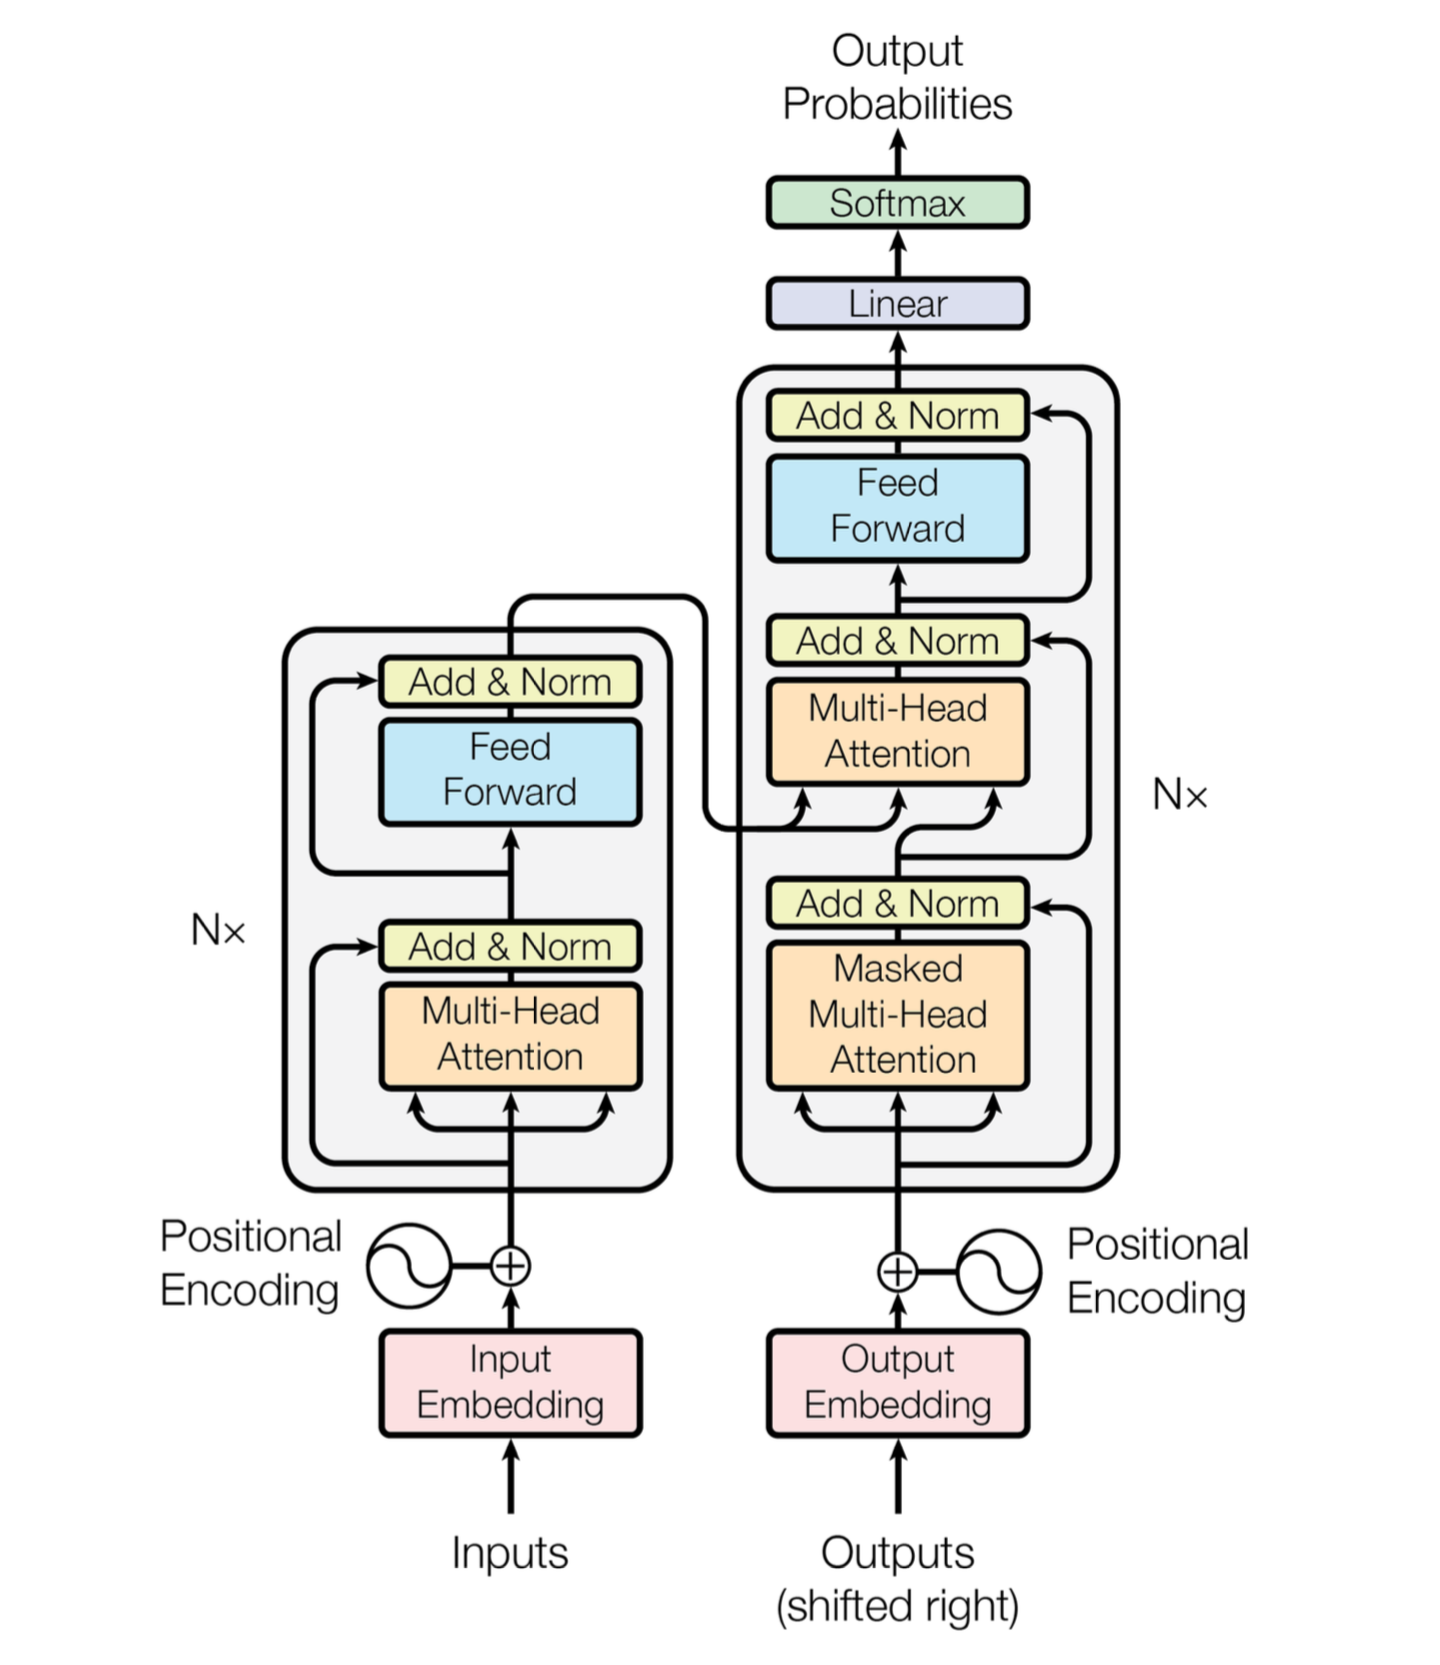
\includegraphics[ width = .3\textwidth]{media/transformer.png}
	% 		\caption{Transformer Model Architecture (Vaswani et al., 2017)}
	% 	\end{subfigure}%
	% 	\begin{subfigure}{.5\textwidth}
	% 		\centering
	% 		
\includegraphics[ width = .3\textwidth]{media/bert-head_orig.jpeg}
	% 		\caption{Transformer Model Architecture (Vaswani et al., 2017)}
	% 	\end{subfigure}
	% \end{figure}
	\begin{figure}[H]
		\centering
		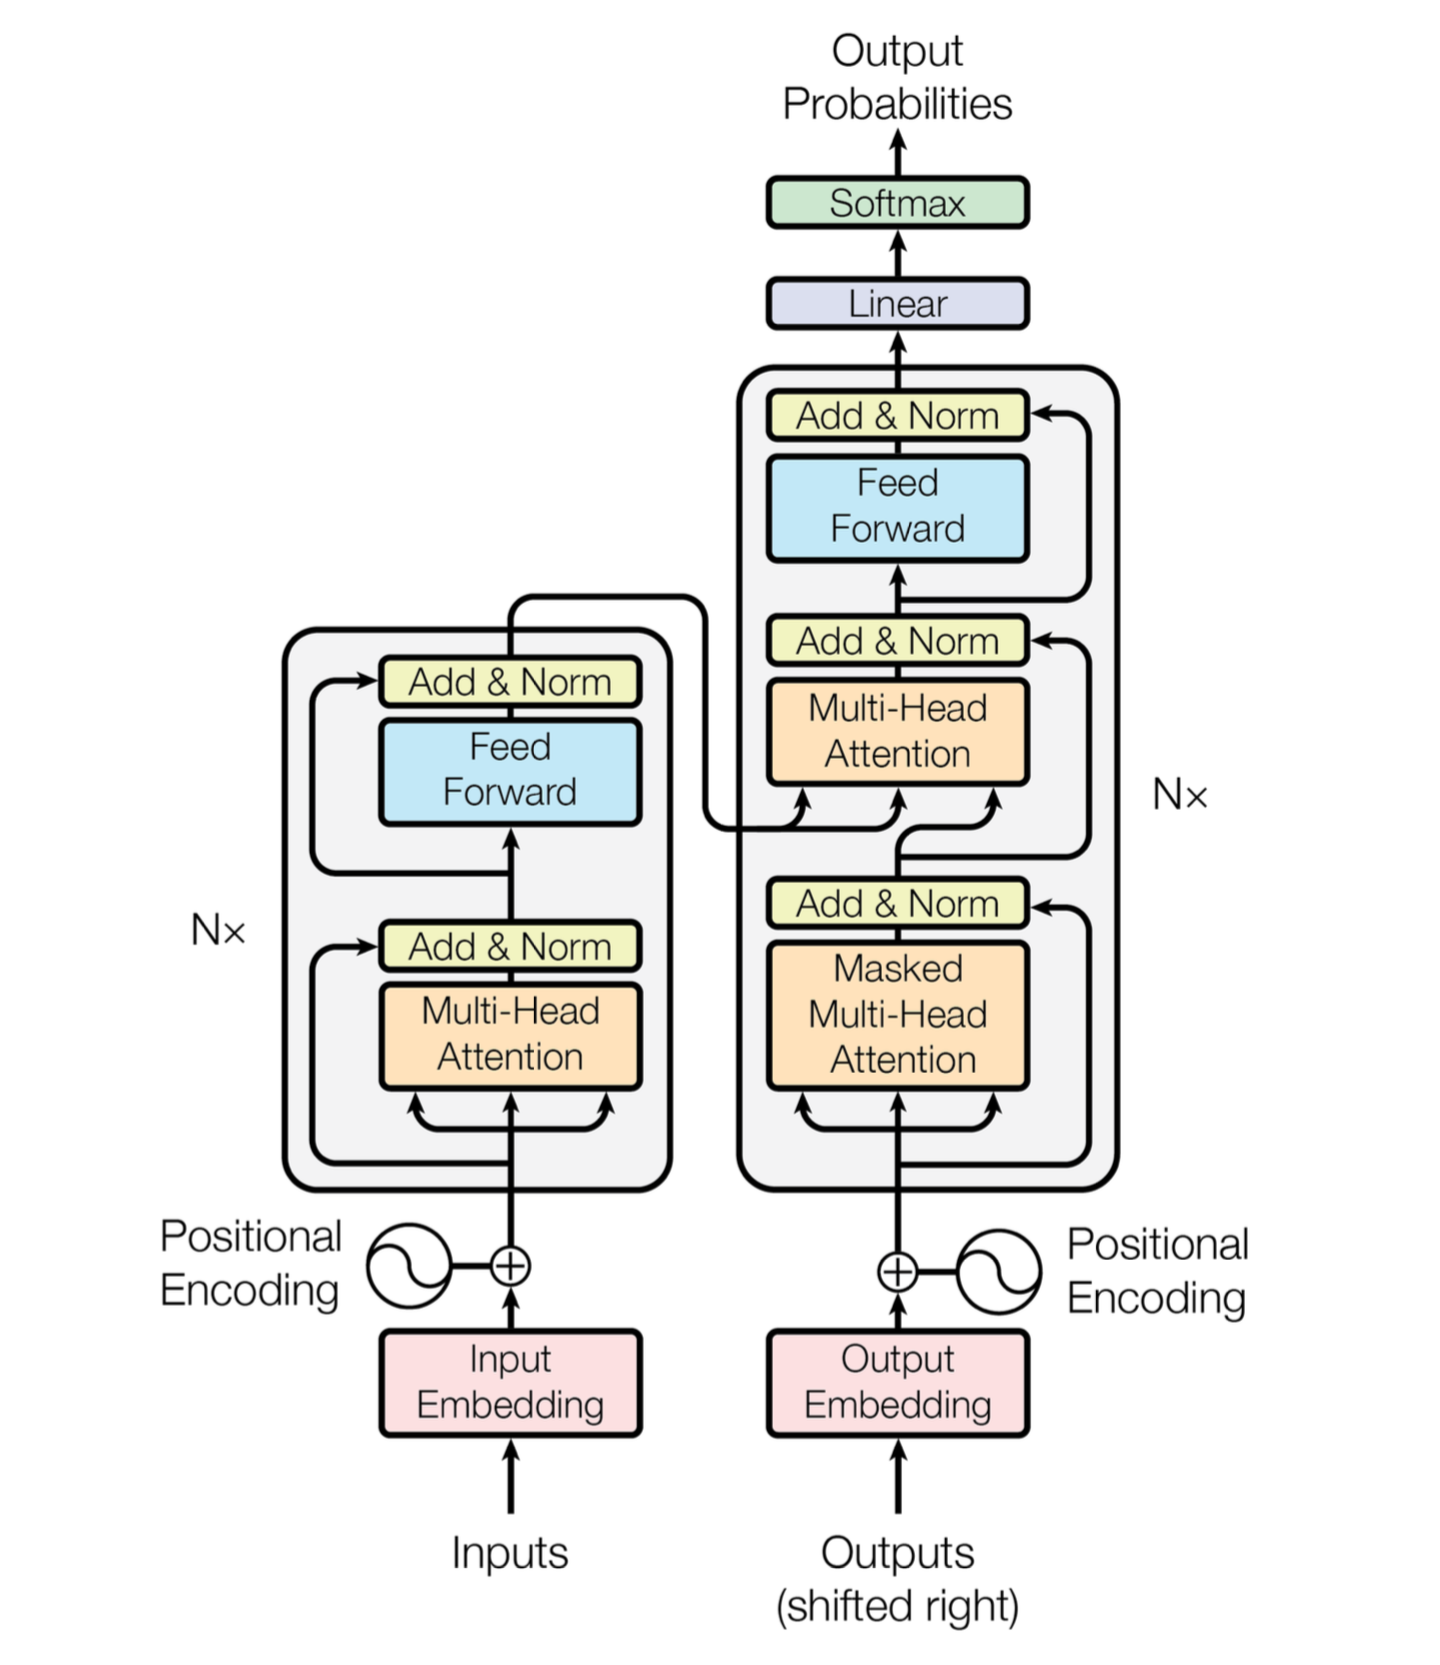
\includegraphics[ width = .35\textwidth]{media/transformer.png}
		\caption{Transformer Model Architecture (Vaswani et al., 2017)}
	\end{figure}


\end{frame}

%Adv Ex
\begin{frame}
	\frametitle{Motivation}
	\framesubtitle{\textbf{Adversarial Examples} Against a BERT ABSA Model}
	\begin{figure}[H]
		\centering
		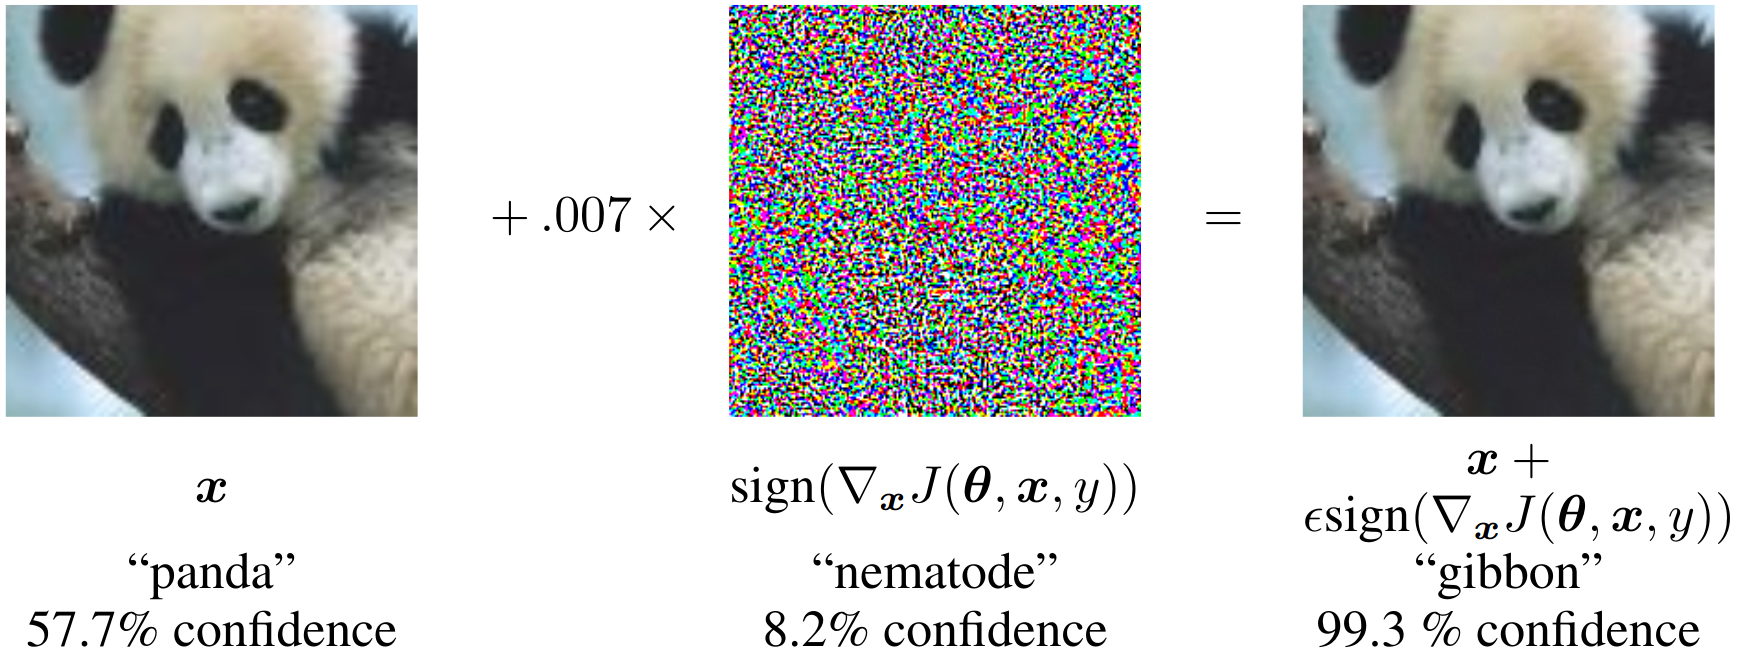
\includegraphics[ width = .8\textwidth]{media/panda.png}
		\caption{Adversarial Examples in Computer Vision (Goodfellow et al, ICLR 2015)}
		%\caption{Source: Explaining and Harnessing Adversarial Examples, Goodfellow et al, ICLR 2015.}
	\end{figure}

\end{frame}

%Autonomous Driving
\begin{frame}
	\frametitle{Motivation}
	\begin{figure}[H]
		\centering
		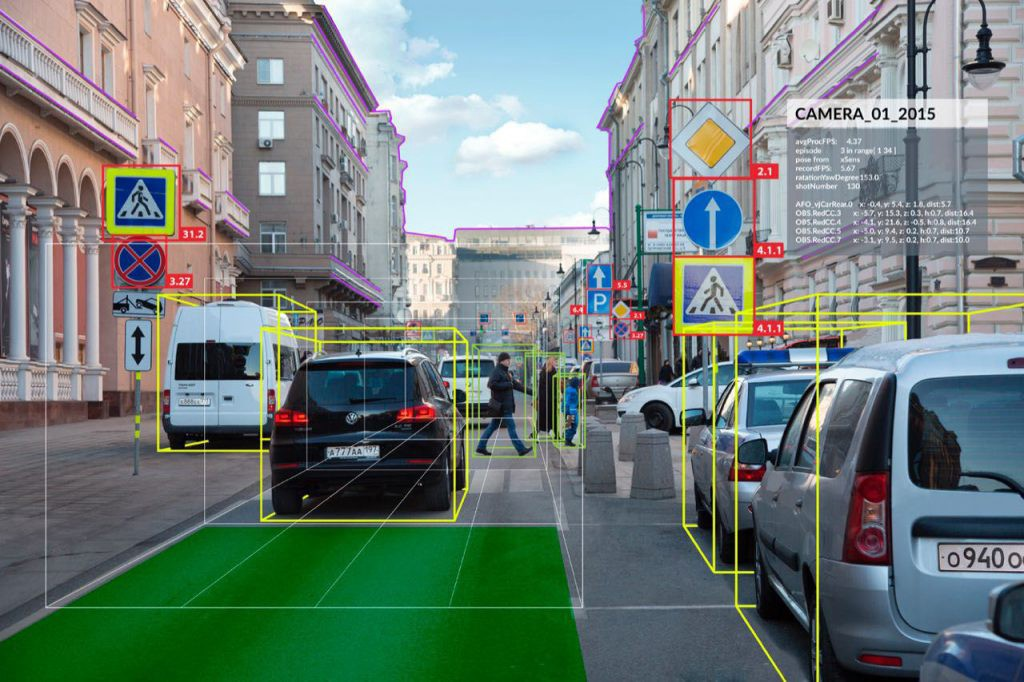
\includegraphics[ width = .625\textwidth]{media/car.png}
		\caption{Object detection in autonomous driving (Source: becominghuman.ai)}
		%\caption{Source: Explaining and Harnessing Adversarial Examples, Goodfellow et al, ICLR 2015.}
	\end{figure}

\end{frame}

%Tweet 
\begin{frame}
	\frametitle{Motivation}
	\begin{figure}[H]
		\centering
		
\includegraphics[ width = .625\textwidth]{media/tweet1.png}
		\caption{Tweet containing misleading information regarding Covid-19, detected and labeled correctly}
		%\caption{Source: Explaining and Harnessing Adversarial Examples, Goodfellow et al, ICLR 2015.}
	\end{figure}

\end{frame}

\begin{frame}
	\frametitle{Motivation}
	\begin{figure}[H]
		\centering
		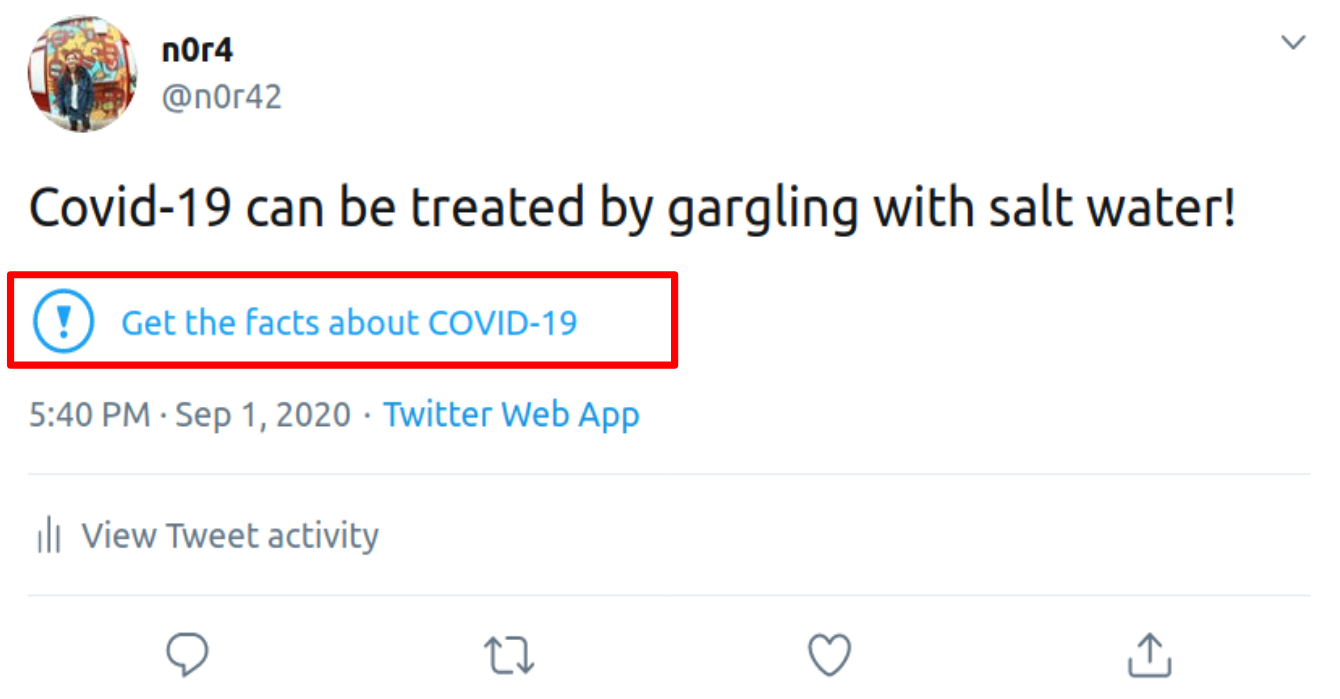
\includegraphics[ width = .625\textwidth]{media/tweet2.png}
		\caption{Tweet containing misleading information regarding Covid-19, detected and labeled correctly}
		%\caption{Source: Explaining and Harnessing Adversarial Examples, Goodfellow et al, ICLR 2015.}
	\end{figure}

\end{frame}

\begin{frame}
	\frametitle{Motivation}
	\begin{figure}[H]
		\centering
		
\includegraphics[ width = .625\textwidth]{media/tweet3.png}
		\caption{Tweet containing misleading information regarding Covid-19. Potential problems due to the use of Leet Speak.}
		%\caption{Source: Explaining and Harnessing Adversarial Examples, Goodfellow et al, ICLR 2015.}
	\end{figure}

\end{frame}


%Adversarial Attacks Motivation Conclusion - Statement Papernot
% \begin{frame}
% 	\frametitle{Adversarial Attacks}
% 	\centering\textit{“We’re starting to deploy machine learning as a technology that can fail so we need to have some checks in place.”}
% 	\centering\textit{Nicolas Papernot, 2017}

% \end{frame}


% Rectangle 1
\begin{frame}[plain]
	\frametitle{Adversarial Attacks against BERT for ABSA}

	\tikzset{every picture/.style={line width=0.75pt}}

	\begin{tikzpicture}[x=0.75pt,y=0.75pt,yscale=-1,xscale=1]

		%Rectangle 1
		\draw  [fill={rgb, 255:red, 224; green, 224; blue, 224 }  ,fill opacity=1 ][line width=0.75]  (94.75,13.45) -- (599.75,13.45) -- (599.75,49.73) -- (94.75,49.73) -- cycle ;
		\draw (228.63,23.59) node [anchor=north west][inner sep=0.75pt]   [align=left] {1. Fine-Tuning BERT base for ABSA};

	\end{tikzpicture}
	\pause
	\\[13pt]
	\centering{Aspect-based Sentiment Analysis}
	\pause
	\\[13pt]


	\begin{columns}[T] % align columns
		\begin{column}{.5\textwidth}
			\begin{minipage}[t]{0.5\linewidth}
				\begin{varblock}[8cm]{Dataset: SemEval-2015 Task 12}
					\begin{itemize}

						\footnotesize\item Labels contain a set of \textbf{Entity - Attribute - Sentiment}
						\item 23 Entities - 9 Attributes - 3 Sentiments (POS, NEG, NEU)
						      \\[7pt]
						\item \textbf{Entity:} reviewd entity
						\item \textbf{Attribute:} particular attribute of an entity
						\item \textbf{Sentiment:} polarity towards the entity and its attribute

					\end{itemize}
				\end{varblock}
			\end{minipage}
		\end{column}%
		\hfill%
		\begin{column}{0.4\textwidth}

			\begin{minipage}[t]{0.8\linewidth}

				\begin{figure}[H]
					\centering
					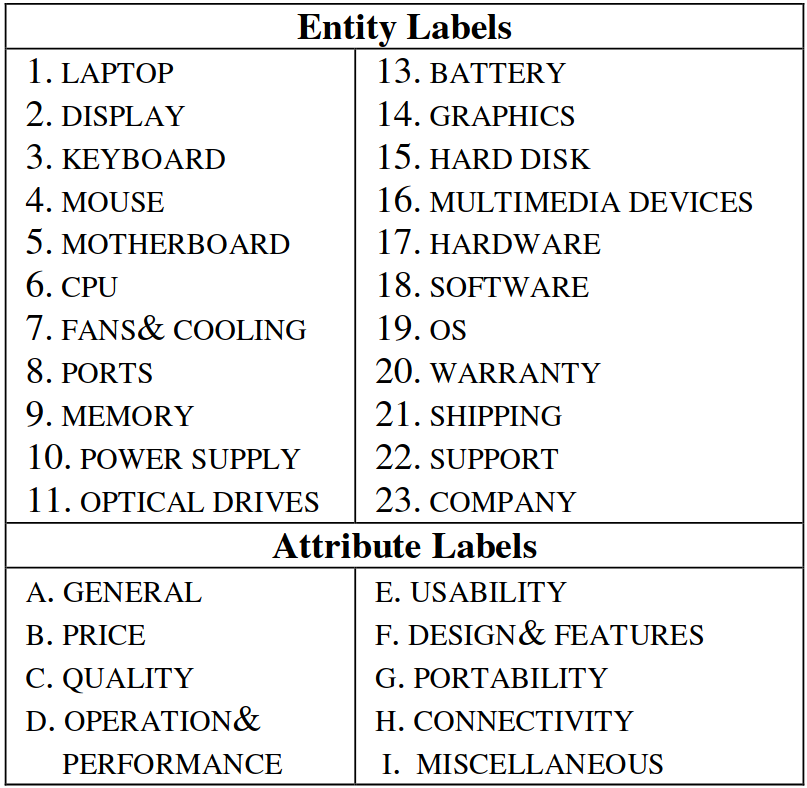
\includegraphics[ width = 1\textwidth]{media/semeval.png}
					%\caption{Laptop Entity Aspect Categproes (Pontiki et al., 2015)}
				\end{figure}

			\end{minipage}
		\end{column}%

	\end{columns}

\end{frame}






% Rectangle 1
\begin{frame}[plain]
	\frametitle{Adversarial Attacks against BERT for ABSA}

	\tikzset{every picture/.style={line width=0.75pt}}

	\begin{tikzpicture}[x=0.75pt,y=0.75pt,yscale=-1,xscale=1]

		%Rectangle 1
		\draw  [fill={rgb, 255:red, 224; green, 224; blue, 224 }  ,fill opacity=1 ][line width=0.75]  (94.75,13.45) -- (599.75,13.45) -- (599.75,49.73) -- (94.75,49.73) -- cycle ;
		\draw (228.63,23.59) node [anchor=north west][inner sep=0.75pt]   [align=left] {1. Fine-Tuning BERT base for ABSA};

	\end{tikzpicture}
	\\[13pt]


	\centering{Aspect-based Sentiment Analysis}
	\\[13pt]

	\centering{\textit{The computer is excellent for gaming but I think it is way too expensive!!}}
	\\[200pt]
\end{frame}

\begin{frame}[plain]
	\frametitle{Adversarial Attacks against BERT for ABSA}

	\tikzset{every picture/.style={line width=0.75pt}}

	\begin{tikzpicture}[x=0.75pt,y=0.75pt,yscale=-1,xscale=1]

		%Rectangle 1
		\draw  [fill={rgb, 255:red, 224; green, 224; blue, 224 }  ,fill opacity=1 ][line width=0.75]  (94.75,13.45) -- (599.75,13.45) -- (599.75,49.73) -- (94.75,49.73) -- cycle ;
		\draw (228.63,23.59) node [anchor=north west][inner sep=0.75pt]   [align=left] {1. Fine-Tuning BERT base for ABSA};


	\end{tikzpicture}
	\\[13pt]
	\centering{Aspect-based Sentiment Analysis}
	\\[13pt]
	\centering{\textit{The computer is \colorbox{YellowGreen}{excellent for gaming} but I think it is \colorbox{Salmon}{way too expensive}!!}}
	\\[13pt]
	\centering{ Aspect: Gaming, Sentiment: POS\\}
	\centering{ Aspect: Price, Sentiment: NEG}
	\\[200pt]

\end{frame}


%Rectangle 2

\begin{frame}[plain]

	\frametitle{Adversarial Attacks against BERT for ABSA}

	\tikzset{every picture/.style={line width=0.75pt}}

	\begin{tikzpicture}[x=0.75pt,y=0.75pt,yscale=-1,xscale=1]

		%Rectangle 1
		\draw  [fill={rgb, 255:red, 224; green, 224; blue, 224 }  ,fill opacity=1 ][line width=0.75]  (94.75,13.45) -- (599.75,13.45) -- (599.75,49.73) -- (94.75,49.73) -- cycle ;
		\draw (228.63,23.59) node [anchor=north west][inner sep=0.75pt]   [align=left] {1. Fine-Tuning BERT base for ABSA};

		%Down Arrow 1
		\draw  [fill={rgb, 255:red, 224; green, 224; blue, 224 }  ,fill opacity=1 ] (319.87,74.92) -- (339.7,74.92) -- (339.7,61.39) -- (354.21,61.39) -- (354.21,74.92) -- (374.05,74.92) -- (346.96,93.06) -- cycle ;

		%Rectangle 2
		\draw  [fill={rgb, 255:red, 224; green, 224; blue, 224 }  ,fill opacity=1 ][line width=0.75]  (94.75,102.84) -- (599.75,102.84) -- (599.75,139.12) -- (94.75,139.12) -- cycle ;
		\draw (259.24,112.98) node [anchor=north west][inner sep=0.75pt]   [align=left] {2. Identify Important Word};

	\end{tikzpicture}
	\\[13pt]
	\pause
	\centering{Leave-One-Out Method}
	\\[13pt]
	\pause
	\begin{tiny}
		\textbf{
			\textit{The computer is \colorbox{YellowGreen}{excellent for gaming}
				but I think it is \colorbox{Salmon}{way too expensive!!}}
		} Gaming - POS; Price - NEG
		\\[13pt]


		\textit{
			\textbf{The}
			- computer is \colorbox{YellowGreen}{excellent for gaming}
			but I think it is \colorbox{Salmon}{way too expensive!!}
		}
		Gaming - POS; Price - NEG
		\\[.5pt]
		\textit{\textbf{computer} - The is \colorbox{YellowGreen}{excellent for gaming} but I think it is \colorbox{Salmon}{way too expensive!!}} Gaming - POS; Price - NEG\\[.5pt]
		\textit{\textbf{is} - The computer \colorbox{YellowGreen}{excellent for gaming} but I think it is \colorbox{Salmon}{way too expensive!!}} Gaming - POS; Price - NEG\\[.5pt]
		\textit{\textbf{excellent} - The computer is for gaming but I think it is \colorbox{Salmon}{way too expensive!!}} Price - NEG\\[.5pt]
		\textit{\textbf{for} - The computer is \colorbox{YellowGreen}{excellent gaming} but I think it is \colorbox{Salmon}{way too expensive!!}} Gaming - POS; Price - NEG \\[.5pt]
		%...
	\end{tiny}
\end{frame}

%Rectangle 3

\begin{frame}[plain]
	\frametitle{Adversarial Attacks against BERT for ABSA}

	\tikzset{every picture/.style={line width=0.75pt}}

	\begin{tikzpicture}[x=0.75pt,y=0.75pt,yscale=-1,xscale=1]

		%Rectangle 1
		\draw  [fill={rgb, 255:red, 224; green, 224; blue, 224 }  ,fill opacity=1 ][line width=0.75]  (94.75,13.45) -- (599.75,13.45) -- (599.75,49.73) -- (94.75,49.73) -- cycle ;
		\draw (228.63,23.59) node [anchor=north west][inner sep=0.75pt]   [align=left] {1. Fine-Tuning BERT base for ABSA};

		%Down Arrow 1
		\draw  [fill={rgb, 255:red, 224; green, 224; blue, 224 }  ,fill opacity=1 ] (319.87,74.92) -- (339.7,74.92) -- (339.7,61.39) -- (354.21,61.39) -- (354.21,74.92) -- (374.05,74.92) -- (346.96,93.06) -- cycle ;

		%Rectangle 2
		\draw  [fill={rgb, 255:red, 224; green, 224; blue, 224 }  ,fill opacity=1 ][line width=0.75]  (94.75,102.84) -- (599.75,102.84) -- (599.75,139.12) -- (94.75,139.12) -- cycle ;
		\draw (259.24,112.98) node [anchor=north west][inner sep=0.75pt]   [align=left] {2. Identify Important Word};

		%Down Arrow 2
		\draw  [fill={rgb, 255:red, 224; green, 224; blue, 224 }  ,fill opacity=1 ] (321.27,164.32) -- (341.1,164.32) -- (341.1,150.78) -- (355.61,150.78) -- (355.61,164.32) -- (375.45,164.32) -- (348.36,182.46) -- cycle ;

		%Rectangle 3
		\draw  [fill={rgb, 255:red, 224; green, 224; blue, 224 }  ,fill opacity=1 ][line width=0.75]  (94.75,194.83) -- (599.75,194.83) -- (599.75,231.11) -- (94.75,231.11) -- cycle ;
		\draw (234.03,204.97) node [anchor=north west][inner sep=0.75pt]   [align=left] {3. Modification of Important Words};
		\pause
		%Rectangle Leet 
		\draw  [fill={rgb, 255:red, 224; green, 224; blue, 224 }  ,fill opacity=1 ][line width=0.75]  (94.75,240.17) -- (258.34,240.17) -- (258.34,276.45) -- (94.75,276.45) -- cycle ;
		\draw (140.85,250.31) node [anchor=north west][inner sep=0.75pt]   [align=left] {Leetspeak};

		%Rectangle Misspellings
		\draw  [fill={rgb, 255:red, 224; green, 224; blue, 224 }  ,fill opacity=1 ][line width=0.75]  (265.34,240.17) -- (428.93,240.17) -- (428.93,276.45) -- (265.34,276.45) -- cycle ;
		\draw (305.63,249.02) node [anchor=north west][inner sep=0.75pt]   [align=left] {Misspellings};

		%Rectangle Punct
		\draw  [fill={rgb, 255:red, 224; green, 224; blue, 224 }  ,fill opacity=1 ][line width=0.75]  (435.92,240.17) -- (599.52,240.17) -- (599.52,276.45) -- (435.92,276.45) -- cycle ;
		\draw (478.42,250.15) node [anchor=north west][inner sep=0.75pt]   [align=left] {Punctuation};

	\end{tikzpicture}

\end{frame}


% Objectives

\begin{frame}
	\frametitle{Adversarial Attacks}

	\begin{block}{Objectives}
		\begin{itemize}

			\item Semantic Meaning
			\item Inconspicousness
			\item Relevance

		\end{itemize}
	\end{block}


\end{frame}


% Leet
\begin{frame}[plain]
	\frametitle{Adversarial Attacks against BERT for ABSA}

	\tikzset{every picture/.style={line width=0.75pt}}

	\begin{tikzpicture}[x=0.75pt,y=0.75pt,yscale=-1,xscale=1]

		%Rectangle 1
		\draw  [fill={rgb, 255:red, 224; green, 224; blue, 224 }  ,fill opacity=1 ][line width=0.75]  (94.75,13.45) -- (599.75,13.45) -- (599.75,49.73) -- (94.75,49.73) -- cycle ;
		\draw (228.63,23.59) node [anchor=north west][inner sep=0.75pt]   [align=left] {1. Leetspeak};
	\end{tikzpicture}
	\\[13pt]

	\begin{small}

		\centering{
			\textit{
				The computer is \colorbox{YellowGreen}{excellent for gaming}
				but I think it is \colorbox{Salmon}{way too expensive!!}
			}}\\[13pt]
		\centering{Aspect: Gaming, Sentiment: POS}\\[.5pt]
		\centering{Aspect: Price, Sentiment: NEG}\\[13pt]



		\centering{
			\textit{
				Original important word:
				\textbf{excellent}
			}
		}

		\centering{
			\textit{
				Modified important word:
				\textbf{
					\color{red}{exce11ent}
				}
			}
		}
		\\[13pt]

		\centering{
			\textit{
				The computer is \colorbox{Salmon}{\color{red}{exce11ent} for gaming}
				but I think it is \colorbox{Salmon}{way too expensive!!}
			}}\\[13pt]
		\centering{Aspect: Gaming, \color{red}{Sentiment: NEG}}\\[.5pt]
		\centering{Aspect: Price, Sentiment: NEG}

	\end{small}

\end{frame}

% Misspellings
\begin{frame}[plain]
	\frametitle{Adversarial Attacks against BERT for ABSA}

	\tikzset{every picture/.style={line width=0.75pt}}

	\begin{tikzpicture}[x=0.75pt,y=0.75pt,yscale=-1,xscale=1]

		%Rectangle 1
		\draw  [fill={rgb, 255:red, 224; green, 224; blue, 224 }  ,fill opacity=1 ][line width=0.75]  (94.75,13.45) -- (599.75,13.45) -- (599.75,49.73) -- (94.75,49.73) -- cycle ;
		\draw (228.63,23.59) node [anchor=north west][inner sep=0.75pt]   [align=left] {2. Misspellings};

	\end{tikzpicture}
	\\[13pt]

	\begin{small}
		\centering{
			\textit{
				The computer is \colorbox{YellowGreen}{excellent for gaming}
				but I think it is \colorbox{Salmon}{way too expensive!!}
			}}\\[13pt]

		\centering{Aspect: Gaming, Sentiment: POS}\\[.5pt]
		\centering{Aspect: Price, Sentiment: NEG}
		\\[13pt]
		\centering{\textit{Original important word: \textbf{excellent}}}\\[.5pt]
		\centering{\textit{Modified important word: \textbf{\color{red}{ecxellent}}}}
		\\[13pt]
		\centering{
			\textit{
				The computer is \color{red}{ecxellent} for gaming
				but I think it is \colorbox{Salmon}{way too expensive!!}
			}}\\[13pt]
		\centering{Aspect: Price, Sentiment: NEG}

	\end{small}

\end{frame}

% Punctuation
\begin{frame}[plain]
	\frametitle{Adversarial Attacks against BERT for ABSA}

	\tikzset{every picture/.style={line width=0.75pt}}

	\begin{tikzpicture}[x=0.75pt,y=0.75pt,yscale=-1,xscale=1]

		%Rectangle 1
		\draw  [fill={rgb, 255:red, 224; green, 224; blue, 224 }  ,fill opacity=1 ][line width=0.75]  (94.75,13.45) -- (599.75,13.45) -- (599.75,49.73) -- (94.75,49.73) -- cycle ;
		\draw (228.63,23.59) node [anchor=north west][inner sep=0.75pt]   [align=left] {3. Punctuation};

	\end{tikzpicture}
	\\[13pt]
	\centering{
		\textit{
			The computer is \colorbox{YellowGreen}{excellent for gaming}
			but I think it is \colorbox{Salmon}{way too expensive!!}
		}}
	\\[13pt]
	\centering{Aspect: Gaming, Sentiment: POS}\\[.5pt]
	\centering{Aspect: Price, Sentiment: NEG}
	\\[13pt]
	\centering{\textit{Original important word: \textbf{excellent}}}\\[.5pt]
	\centering{\textit{Modified important word: \textbf{\color{red}{excellent,}}}}
	\\[13pt]
	\centering{
		\textit{
			The \colorbox{YellowGreen}{computer is \color{red}{excellent,}}\colorbox{Salmon}{ for gaming
				but I think} it is \colorbox{Salmon}{way too expensive!!}
		}}
	\\[13pt]
	\centering{\color{red}{Aspect: Laptop (general), Sentiment: NEG}}\\[.5pt]
	\centering{Aspect: Gaming, \color{red}{Sentiment: NEG}}\\[.5pt]
	\centering{Aspect: Price, Sentiment: NEG}



\end{frame}

%todo: onslide one after the other column..
% Results Total
\begin{frame}
	\frametitle{Qualitative Results}

	\begin{table}[ht]
		\centering
		\resizebox{.85\textwidth}{!}{%
			\begin{tabular}{lccc}
				\toprule
				\onslide<0->\textbf{Perturbation Method}                                                             \onslide<0-> & \textbf{Leetspeak}              \onslide<0-> & \textbf{ Misspellings}                           \onslide<0-> & \textbf{Punctuation} \\ \midrule
				\onslide<1->Dataset A - \# of original sentences                			\onslide<1->                                      & 943               \onslide<1->               & 943                                 \onslide<1->              & 943                  \\ %\hline
				\onslide<2->Dataset B - \# of modifiable original sentences                 \onslide<2->                          & 897                \onslide<2->              & 369                    \onslide<2->                           & 943                  \\ %\hline
				\onslide<3->Dataset C - \# of adversarial sentences                         \onslide<3->                          & 2232               \onslide<3->              & 1354                   \onslide<3->                           & 2555                 \\ %\hline
				\onslide<4->Dataset D - \# of changed predictions total                     \onslide<4->                          & 1066               \onslide<4->              & 420                    \onslide<4->                           & 382                  \\ %\hline
				\onslide<4->Dataset E - \# of changed predictions per sentence              \onslide<4->                          & 790                \onslide<4->              & 259                    \onslide<4->                           & 253                  \\ \midrule
				\onslide<5->\textbf{Overall Success Rate}                                   \onslide<5->                          & \textbf{47.76\%}   \onslide<5->              & \textbf{31.01\%}       \onslide<5->                           & \textbf{14.95\%}     \\ \bottomrule
				\onslide<5->\textbf{Distinct Success Rate}                                  \onslide<5->                          & \textbf{88.07\%}   \onslide<5->              & \textbf{70.19\%}       \onslide<5->                           & \textbf{26.83\%}     \\ \bottomrule
			\end{tabular}%
		}
		\caption{Comparison of the success rates of the three attack methods.}

	\end{table}
\end{frame}

% Conclusion
\begin{frame}
	\frametitle{Conclusion \& Further Steps}
	\begin{block}{Summary}
		\begin{itemize}
			\item BERT can be fooled by input modofications
			\item Three attack methods:
			      \begin{itemize}
				      \item Leetspeak
				      \item Misspellings
				      \item Falsly placed Punctuation
			      \end{itemize}
		\end{itemize}
	\end{block}
	\begin{block}{Next Steps}
		\begin{itemize}
			\item Transferability between Transformer Models
			\item Using generated adversarial datasets for Adversarial Training

		\end{itemize}
	\end{block}

\end{frame}

% Personal
\begin{frame}
	\frametitle{Thank you!}
	\textit{Adversarial Examples Against A BERT ABSA Model -
		\\[13pt]
		Fooling BERT with L\colorbox{Salmon}{33T}, Misspelli\colorbox{Salmon}{gn}, and Punctuation\colorbox{Salmon}{,}
	}
	\\[20pt]

	%todo: add icons
	%https://latexdraw.com/fontawesome-ready-icons-to-use-in-latex/
	% no idea why this is not working
	\textbf{Github:} https://github.com/NoraH2004/adv-absa
	\\[5pt]
	\textbf{Email:} nora.hofer@uibk.ac.at
\end{frame}




% Titlepage - FIN
\begin{frame}
	\titlepage
\end{frame}


\end{document}
